\documentclass[conference]{IEEEtran}
\IEEEoverridecommandlockouts
\usepackage{microtype}
\usepackage{flushend}
\usepackage{cite}
\usepackage{float}
\usepackage[table]{xcolor}
\usepackage{amsmath,amssymb,amsfonts}
\usepackage{algorithmic}
\usepackage{graphicx}
\usepackage{textcomp}
\usepackage{xcolor}
\def\BibTeX{{\rm B\kern-.05em{\sc i\kern-.025em b}\kern-.08em
    T\kern-.1667em\lower.7ex\hbox{E}\kern-.125emX}}
\usepackage{tabularx}
\usepackage[vietnamese, english]{babel}
\usepackage{array}
\usepackage[utf8]{inputenc}
\usepackage[T1]{fontenc}
\usepackage{amsmath}
\usepackage{amsfonts}
\usepackage{amssymb}
\usepackage[version=4]{mhchem}
\usepackage{stmaryrd}
\usepackage{hyperref}
\hypersetup{colorlinks=true, linkcolor=blue, filecolor=magenta, urlcolor=cyan,}
\urlstyle{same}
\usepackage[export]{adjustbox}
\graphicspath{ {./images/} }
\usepackage{multirow}
\usepackage{booktabs}
\usepackage{caption}
\usepackage{siunitx}
\usepackage{array}
\newcolumntype{L}{>{\raggedright\arraybackslash}X}

\raggedbottom
\title{Forecasting Stock Prices of Sneaker Brands*}

\author{\IEEEauthorblockN{1\textsuperscript{st} Vu Quoc Tuan}
\IEEEauthorblockA{\textit{STAT3013.012.CTTT} \\
\textit{University of Information Technology}\\
Ho Chi Minh \\
21522767@gm.uit.edu.vn}
\and
\IEEEauthorblockN{2\textsuperscript{nd} Nguyen Thanh Nhan}
\IEEEauthorblockA{\textit{STAT3013.012.CTTT} \\
\textit{University of Information Technology}\\
Ho Chi Minh \\
21522404@gm.uit.edu.vn}
\and
\IEEEauthorblockN{3\textsuperscript{rd} Mai Dang Minh}
\IEEEauthorblockA{\textit{STAT3013.012.CTTT} \\
\textit{University of Information Technology}\\
Ho Chi Minh \\
21522340@gm.uit.edu.vn}
}


\begin{document}
\maketitle

\begin{abstract}
The fashion industry, especially with major brands such as Nike, Puma and Adidas, plays an important role in the economy and meets the needs of the global fashion market. However, this industry also faces many formulas and traps. One of the biggest formulas that is likely to be expected and effectively handled in the direction of the market.

In the past, the fashion production process often depended on the creativity and experience of designers informed by observation and monitoring of market trends. However, this process is inefficient and sometimes costly in terms of time and resources. For leading fashion brands, the use of data analysis techniques and market trend forecasting is becoming increasingly important.

By applying time series analysis and data modeling methods, the fashion industry can accurately analyze and expect market trends. This research can apply 10 algorithms to predict the development of three famous fashion brands and make important contributions to improving business strategic management and ensuring the sustainability of fashion resources. space. Through the application of these algorithms, it is possible to provide the necessary information to quickly initiate the transformation of the fashion market and maintain the competitiveness of leading brands.
\end{abstract}

\section*{I. INTRODUCTION}
The stock market, with its dynamic and often unpredictable nature, has become a focal point for investors looking for opportunities as well as challenges. Against this backdrop, shares of globally recognized sports apparel and footwear giants, namely Nike, Puma and Adidas, are attracting significant attention. These companies, each with its own market position and strategy, represent key players in the competitive sports and lifestyle industry.

Investors, financial analysts and enthusiasts are all very interested in predicting the future performance of these companies' stocks. The stock prices of Nike, Puma and Adidas are influenced by many factors, including market trends, economic indicators, consumer preferences and global events. Understanding and forecasting these dynamics is critical to making informed investment decisions.

Forecasting sales of famous brands such as Nike, Puma and Adidas is an important part of business strategy, helping to ensure the efficiency and sustainability of the business. This study focuses on predicting the sales of these three brands to provide useful information and support business management in the fashion and sports sectors.

We apply a series of forecasting algorithms, including Autoregressive Integrated Moving Average (ARIMA), Seasonal Autoregressive Integrated Moving Average with eXogenous factors (SARIMAX), Linear regression (LR), Support Vector Regression (SVR), Kalman Filter (KF), Bagging Gated Recurrent Unit (Bagging-GRU), Long Short-Term Memory (LSTM), Simple Exponential Smoothing (SES) . This helps us evaluate and compare the performance of forecasting models in predicting sales of Nike, Puma, and Adidas.

In this way, this study aims to provide insights and strategies to improve the business management of leading sports and fashion stores. Forecasting sales helps them adapt quickly to market fluctuations, optimize marketing and supply strategies, and minimize risks in business management.

\section*{II. RELATED REASEARCH}
\textbf{Linear Regression} - Whereas Müller-Wirtz et al used simple linear regression to address their research question, researchers often need to specify a multivariable model and make choices on which independent variables to include and on how to model the functional relationship between variables (eg, straight line versus curve; inclusion of interaction terms).
Variable selection is a much-debated topic, and the details are beyond the scope of this Statistical Minute. Basically, variable selection depends on whether the purpose of the model is to understand the relationship between variables or to make predictions. This is also predicated on whether there is informed a prior theory to guide variable selection and on whether the model needs to control for variables that are not of primary interest but are confounders that could distort the relationship between other variables[1].\\

\textbf{SARIMAX} - In the research work of two authors F. R. Alharbi and D. Csala on the SARIMAX model in forecasting the long-term power industry by developing a long-term forecasting model that takes into account the impact of energy production and consumption. , maximum load and installed capacity. Experimental results using error indices such as RMSE, MAE, MSE, MAPE demonstrate the effectiveness of the model for all three types of data. The SARIMAX model was also compared with 11 other prediction models, and the results confirmed the superior performance of SARIMAX. For example, the highest RMSE value for the four types of electricity data is 1.2 TWh for generation, and the lowest is 0.2 GW for installed capacity [2]

\textbf{SVR} - The article by M. Wautersa, M. Vanhoucke shows that when the original trainer test set, the Support Vector Regression (SVR) model outperforms other forecasting methods across many levels and Monte Carlo simulation settings . SVR can improve performance over time as the project evolves. While the SVR model is a “garbage in, garbage out” approach, the Project Manager requires the project manager to understand the next dynamic [3]

\textbf{ARIMA, SES} - According to a research article by author Everette S. Gardner Jr., simple exponential smoothing is considered one of the most reliable forecasting methods, demonstrating strong performance on a wide variety of series that do not follow an equivalent ARIMA(0, 1, 1) process. . This includes the common first-order autoregressive processes and some lower-order ARIMA processes. Bossons (1966) emphasized the robustness of simple smoothing, especially its insensitivity to specification errors, especially when the error occurs due to an incorrect belief in the stationarity of the generation process. . Additional research by Hyndman (2001) shows that ARIMA model selection errors can lead to inflated mean squared errors (MSE) compared to simple smoothing performance. In Hyndman's simulation, the time series is generated from the ARIMA process (0, 1, 1) and a set of constrained ARIMA models [(0, 1, 1), (1, 1, 0) and (1, 1, 1)], each with and without a constant term, was fitted. Model selection was performed using Akaike's Information Criterion (AIC) (Akaike, 1970). ARIMA's forecast MSEs are significantly larger than those obtained through simple smoothing due to incorrect model selection, with the problem exacerbated when errors deviate from a normal [4]

\textbf{LSTM} - The research paper by Chung, Gulcehre, Cho, and Bengio, titled "Empirical Evaluation of Gated Recurrent Neural Networks on Sequence Modeling," is a significant contribution in the field of recurrent neural networks, particularly focusing on the LSTM model. The research not only focuses on LSTM but also compares its performance with other models, especially traditional Recurrent Neural Networks (RNNs). This helps clarify the advantages of the gated mechanism in LSTM. The study concludes by praising the capabilities of LSTM in modeling time sequences, particularly when compared to traditional RNN models. It provides deep insights into how LSTM operates on specific tasks and why it is suitable for various time sequence applications. [5]

III. DATA AND METHODOLOGY.

\subsection*{A. Dataset statistics}
Three datasets are about the Sneaker Companies Stock from 02/01/2019 to 28/12/2023 from \textbackslash{}href\{https://finance.yahoo.com/lookup?s=DATA\}{finance.yahoo.com\}, NIKE[6], PUMA[7], ADDIDAS[8]. The datasets include seven attributes columns, Date, Open, High, Low, Close, Adj Close, Vol. 

The primary focus of this study is to identify and employ optimal predictive models for forecasting the "Close" value precisely 30 days into the future, specifically targeting the date 29/01/2024 (originating from the last data point on 28/12/2023). This predictive modeling aims to contribute valuable insights into the future stock performance of these prominent sneaker companies, facilitating informed decision-making in the financial domain.
\begin{table}[htbp]
\centering
\begin{tabular}{|c|c|c|c|} \hline 

 Value& Nike & Puma& Adidas\\ \hline 

 Count& 1258 & 1266& 1258\\ \hline 

 Mean& 114.5519& 69.9389& 127.5647\\ \hline 

 Variance& 635.5032& 309.6534& 1345.5764\\ \hline 

 Standard deviation& 25.2091& 17.5969& 36.682\\ \hline 

 Median & 109.33 & 66.625& 134.605\\ \hline 

 Max& 177.5099& 114.6999& 198.6799\\ \hline 

 Min& 62.7999& 42.1399& 45.50 \\ \hline 

 Mode & 83.9499& 67.4499& 150.66 \\ \hline 

 Quantile 1 & 93.6824& 55.3499& 94.2324\\ \hline 

 Quantile 3 & 132.2175& 82.285& 158.5975\\ \hline 

 Coefficient of deviation& 0.22 & 0.2516& 0.2875\\ \hline 

 Kurtosis & -0.5275& -0.5322& -1.1886\\ \hline 

 Skewness & 0.5514& 0.6868& -0.2001\\ \hline

\end{tabular}
\caption{Overview of descriptive statistics for the three surveyed stores close}
\end{table}
According to Table I, based on the statistical data of 3 Nike, Puma and Adidas stores, we can draw some important observations about their business performance.

All three stores have a large number of observations, however, there is a significant difference in the average product value. While Nike and Adidas show stability with relatively high average values, Puma stands out with low average values. This may indicate that Nike and Adidas are primarily focused on providing high-value products.

If you look at the volatility of the data, Nike and Puma typically have low standard deviations, indicating uniformity in size and little volatility. In contrast, Adidas is highly volatile, possibly due to the variety of products it offers.

When looking at the data distribution, Nike and Puma tend to distribute the data with peaks below the average, creating a skew to the left. Meanwhile, Adidas leans to the right, with most of its value concentrated above average.

These characteristics can help businesses better understand the characteristics and business strategies of each store. Nike and Puma, with their stable nature, can focus on a broad reach strategy, while Adidas, with their high volatility and variety, can focus on unique and focused product development. into the high quality market.

\begin{center}
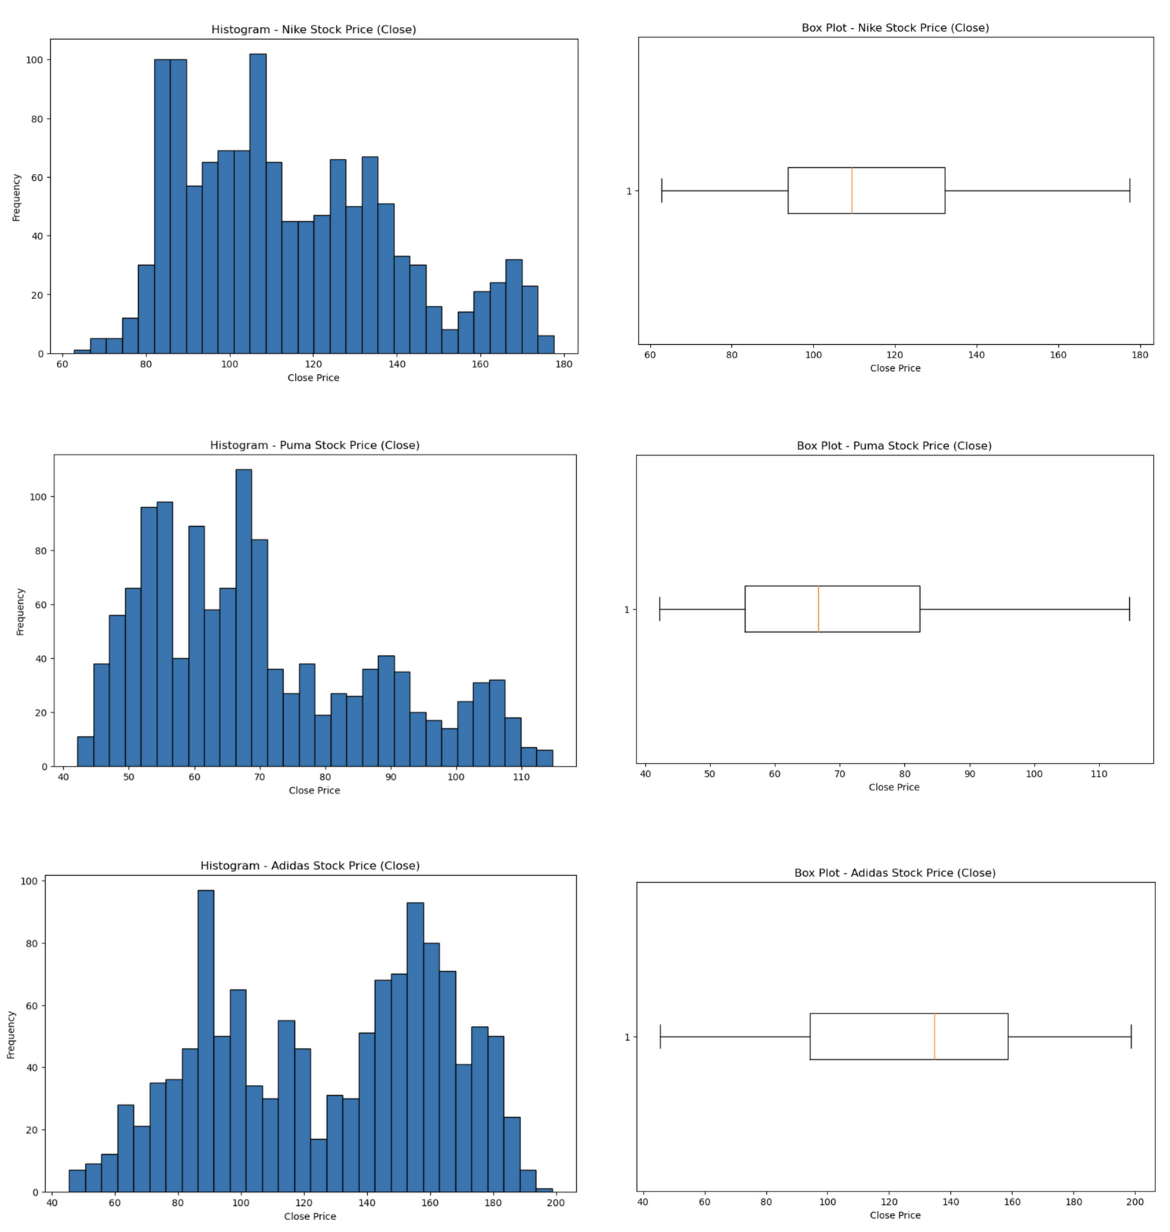
\includegraphics[max width=\linewidth, height = 5cm]{Plot.png}
\end{center}
Figure 1. Histogram and Box plot chart of three stores
\subsection*{B. Measurement}
\setlength{\parskip}{0pt}
The essential step in any machine learning model is to evaluate the accuracy of the model. The Mean Squared Error (MSE), Mean absolute error (MAE), Root Mean Squared Error(RMSE), and Mean Absolute Percentage Error (MAPE). MAE represents the average of the absolute difference between the actual and predicted values in the dataset. It measures the average of the residuals in the dataset. MSE represents the average of the squared difference between the original and predicted values in the data set. It measures the variance of the residuals. While Root Mean Squared Error is the square root of Mean Squared error. It measures the standard deviation of residuals[9]. And MAPE is a metric that defines the accuracy of a forecasting method. It represents the average of the absolute percentage errors of each entry in a dataset to calculate how accurate the forecasted quantities were in comparison with the actual quantities. The equations for these measures are as follows [10]:\\
\begin{gather*}
\text{MSE} = \frac{1}{m} \sum_{i=1}^{m}(X_{i}-Y_{i})^{2} \\
\text{MAPE} = \frac{1}{m} \sum_{i=1}^{m}\left\lvert\frac{Y_{i}-X_{i}}{Y_{i}}\right\rvert
\end{gather*}
\begin{gather*}
\text{MAE} = \frac{1}{m} \sum_{i=1}^{m}\lvert X_{i}-Y_{i} \rvert 
\end{gather*}
\begin{gather*}
\text{RMSE} = \sqrt{\frac{1}{m} \sum_{i=1}^{m}(X_{i}-Y_{i})^{2}} \\
\end{gather*}

Where $\mathrm{m}$ is the number of data points, $X_{i}$ is the predicted $i^{\text {th }}$ value and $Y_{i}$ element is the actual $i^{\text {th }}$ value.

\subsection*{C. Modeling}
\subsubsection*{\textbf{1) Linear Regression} (LR)}
Linear regression analysis is used to predict the value of a variable based on the value of another variable. The variable you want to predict is called the dependent variable. The variable you are using to predict the other variable's value is called the independent variable. Linear regression fits a straight line or surface that minimizes the discrepancies between predicted and actual output values. There are simple linear regression calculators that use a "least squares" method to discover the best-fit line for a set of paired data. You then estimate the value of $\mathrm{X}$ (dependent variable) from $\mathrm{Y}$ (independent variable).[11]

In a simple linear regression, there is one independent variable and one dependent variable. The model estimates the slope and intercept of the line of best fit, which represents the relationship between the variables. The slope represents the change in the dependent variable for each unit change in the independent variable, while the intercept represents the predicted value of the dependent variable when the independent variable is zero.

Linear regression is a quiet and the simplest statistical regression method used for predictive analysis in machine learning. Linear regression shows the linear relationship between the independent(predictor) variable i.e. X-axis and the dependent(output) variable i.e. Y-axis, called linear regression. If there is a single input variable X(independent variable), such linear regression is simple linear regression.[12]

The following is an example of a resulting linear regression equation:

$$
Y=\beta_{0}+\beta_{1} X_{1}+\ldots
$$

\begin{itemize}
  \item $\quad Y:$ The dependent variable.
  \item $\quad X:$ The independent variable.
  \item $\beta_{0}$ : The intercept or the value of $Y$ when other parameters equal zero.
  \item $\beta_{0}$ : The coefficient effect on $\mathrm{X}_{1}$.
\end{itemize}

\begin{center}
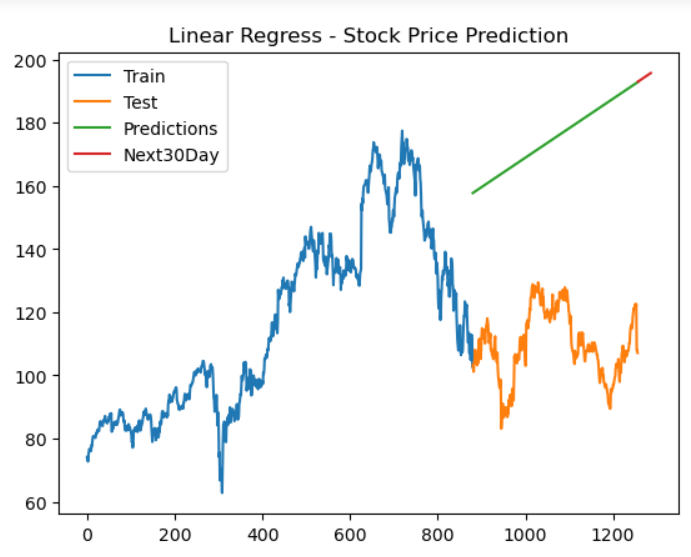
\includegraphics[width=\linewidth, height = 5cm, center]{LR.png}
Figure 2. Result of Linear Regression with NIKE divided by 7-3 ratio.
\end{center}


\begin{table}[H]
\centering
\begin{tabularx}{\columnwidth}{|c|c|X|X|X|X|}
\hline
Model & \begin{tabular}{c}
Train- \\
Test
\end{tabular} & MSE & RMSE & MAE & MAPE \\
\hline
\multirow{3}{*}{LR} & $7-3$ & 4525.835 & 67.2743 & 65.6534 & 0.614 \\
\cline{2-6}
 & $8-2$ & 1503.51 & 38.7751 & 36.4513 & 0.3372 \\
\cline{2-6}
 & $9-1$ & 1331.788 & 36.4936 & 35.797 & 0.3468 \\
\hline
\end{tabularx}
\end{table}
Table II. \textit{Nike-Closing Price} measure result after using $LR$.\\
\subsubsection*{\textbf{2) Simple Exponential Smoothing} (SES)}

The Single Exponential Smoothing (SES) model is a technique employed in time series prediction, aiming to forecast suitable values for a set of variables by relying on predefined survey values. Charles C. Holt, in collaboration with Albert G. Winters, introduced the SES model during the 1950s. It can be viewed as a specific instance within the ETS (Error, Trend, Seasonality) framework, focusing specifically on the Error (E) factor and omitting the consideration of Trend (T) and Seasonality (S) factors. Let’s represent this mathematically, [13]
\textbf{\begin{align*}
f_t = \alpha d_{t-1} + (1 - \alpha)  f_{t-1}, 0 < \alpha <1  
\end{align*}}
\begin{itemize}
    \item \(\alpha\): is a ratio (or a percentage) of how much importance the model will allocate to the most recent observation compared to the importance of demand history.

    \item \(\alpha d_t-1\): represents the previous demand observation times the learning rate. You could say that the model attaches a certain weight (alpha) to the last demand occurrence.

    \item \((1 - \alpha)  f_{t-1}\): represents how much the model remembers from its previous forecast. Note that this is where the recursive magic happens as f\{t-1\} was itself defined as partially d\{t-2\} and f\{t-2\}.
\end{itemize}

But SES is only suitable for simple and stable problems, but is not a good choice when facing complex and volatile time series. In these cases, complex forecasting models often yield better results

\begin{H}
    \centering
    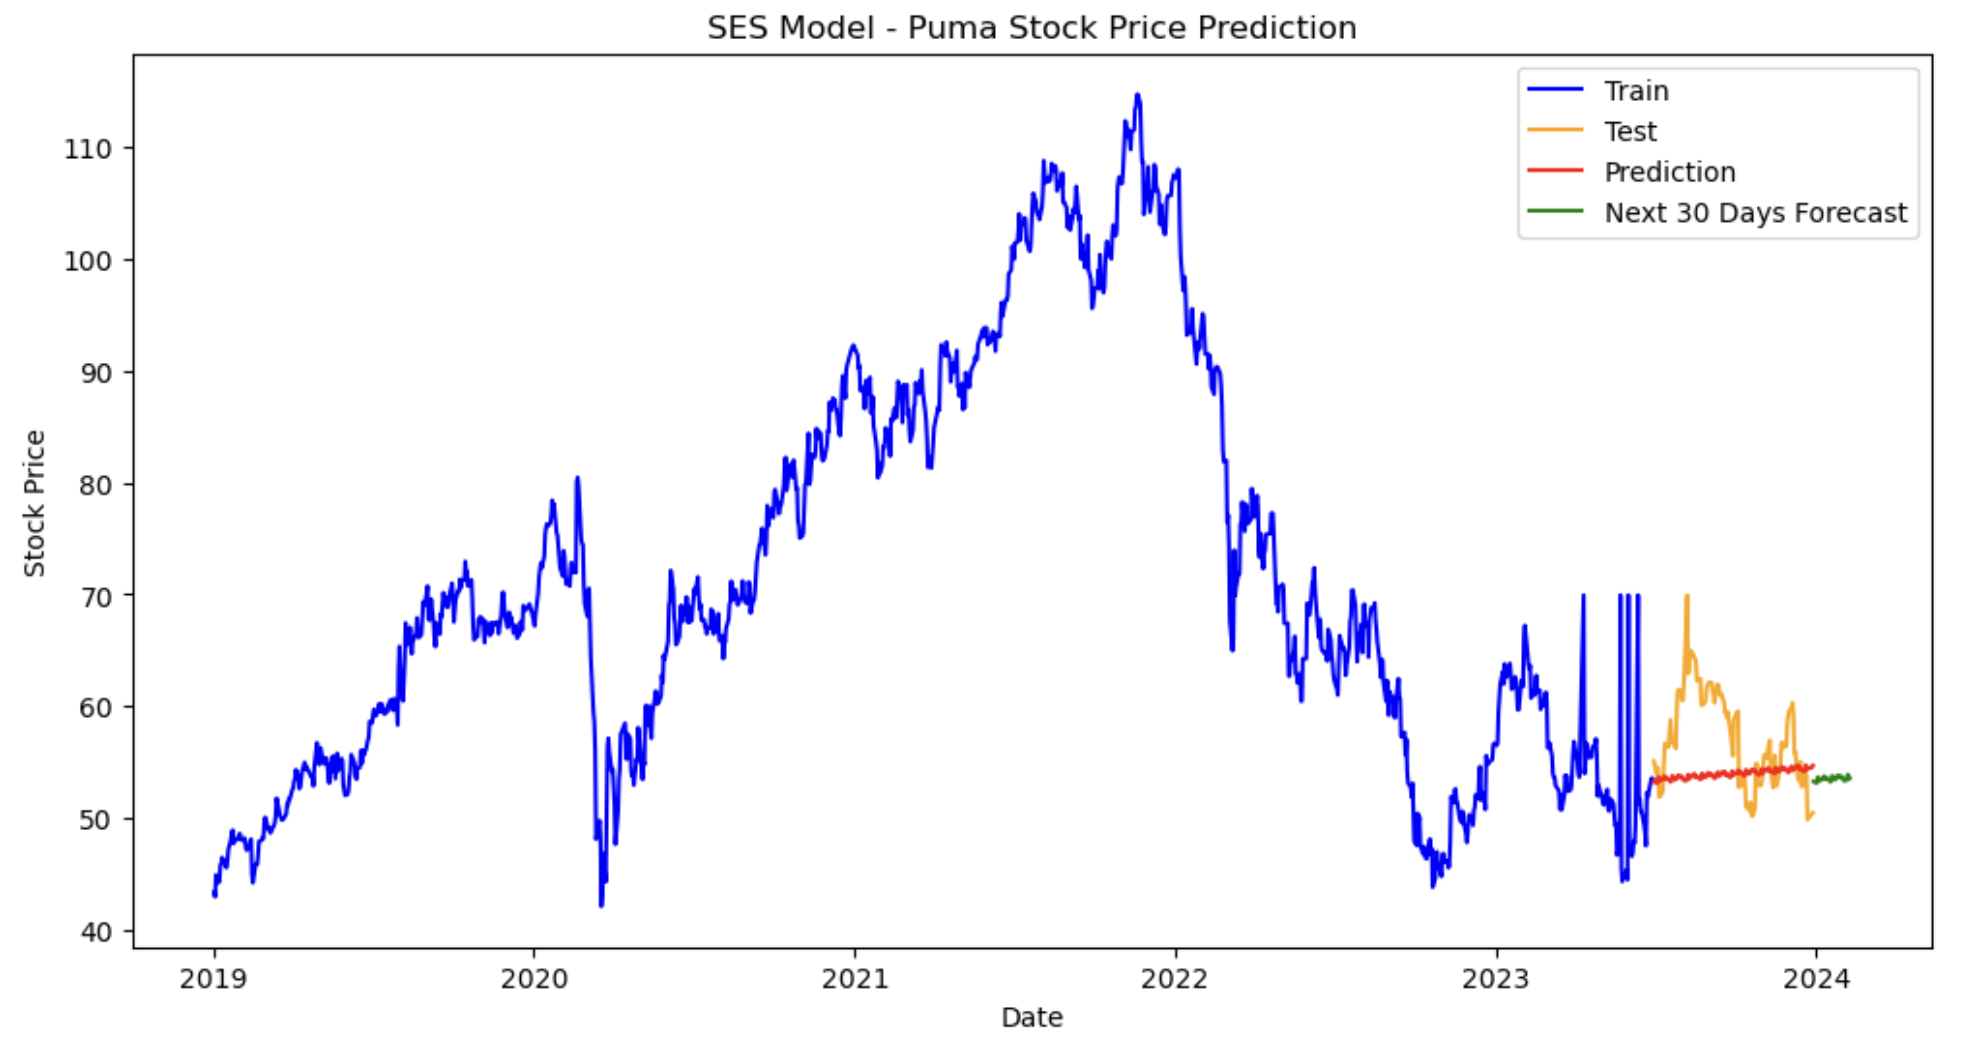
\includegraphics[max width= \linewidth]{SES(PUMA).png}
Figure 3. Result of SES with Puma divided by 9-1 ratio
    \label{fig:enter-label}
\end{H}

\begin{table}[H]
\centering
\begin{tabularx}{\columnwidth}{|c|c|X|X|X|X|}
\hline
Model & \begin{tabular}{c}
Train- \\
Test
\end{tabular} & MSE & RMSE & MAPE & MAE \\
\hline
\multirow{3}{*}{SES} & $7-3$ & 128.94 & 18.87 & 11.36 & 9.98 \\
\cline{2-6}
 & $8-2$ & 32.18 & 8.76 & 5.67 & 4.79 \\
\cline{2-6}
 & $9-1$ & 28.47 & 7.03 & 5.34 & 4.20 \\
\hline
\end{tabularx}
\end{table}
Table III. \textit{Puma-Closing Price} measure result after using $SES$.\\




\subsubsection*{\textbf{3) Autoregressive Integrated Moving Average (ARIMA)}}
ARIMA models consists of three main components:the Auto Regression (AR) component, the Moving Average (MA) component, the Integrated (I) component.

\begin{itemize}
  \item AR: Auto regressive: A model that shows the changing variable that regresses on its own lagged, or prior, value.

  $y(t) = a_0 + a_1 y(t - 1) + \dots + a_p y(t - p) + e(t)$
  
  \begin{flushleft}
    \textbf{Where:}
    \begin{itemize}
      \item $y(t)$ is the current observed value.
      \item $y(t - 1), \dots , y(t - p)$ are past observed values (typically using no more than 2 of past variables).
      \item $a_0, a_1, \dots , a_p$ are regression analysis parameters.
      \item $e(t)$ is the random forecasting error of the current period. The expected mean value is 0.
      \item $y(t)$ is a linear function of the past observed values $y(t - 1), \dots , y(t - p)$.
    \end{itemize}
  \end{flushleft}
  
  \item I: Integrated. Represents the difference of raw observations to allow the time series to become stationary (i.e., data values are replaced by the difference between the data values and the previous values). \\
   First Difference I(1): z(t) = y(t) - y(t - 1) \\
    Second Difference I(2): h(t) = z(t) - z(t - 1)  \\
  \item MA: Moving Average. Incorporates the dependency between an observation and a residual error from a moving average model applied to lagged observations.
  $y(t) = b_0 + e(t) + b_1e(t - 1) + \dots + b_qe(t - q)$
  
  \begin{flushleft}
    \textbf{Where:}
    \begin{itemize}
      \item $y(t)$ is the current observed value.
      \item $e(t)$ is the random forecasting error of the current period. The expected mean value is 0.
      \item $e(t - 1), \dots , e(t - p)$ are forecast error (typically using no more than 2 of past variables).
      \item $b_0, b_1, \dots , b_p$ mean value of $y(t)$ and moving average coefficients.
      \item $q$ is the number of past errors used in the moving average.
    \end{itemize}
  \end{flushleft}
\end{itemize}
An autoregressive integrated moving average, or ARIMA, is a statistical analysis model that uses time series data to either better understand the data set or to predict future trends. Or a statistical model is auto regressive if it predicts future values based on past values.
Each component in ARIMA functions as a parameter with a standard notation.
For ARIMA models, a standard notation would be ARIMA with $\mathrm{p}, \mathrm{d}$, and $\mathrm{q}$ (corresponding to AR, I,MA), where non-negative integer values substitute for the parameters to indicate the type of ARIMA model used.[14]

The parameters can be defined as:

\begin{itemize}
  \item $\mathrm{p}$ : the number of lag observations in the model, also known as the lag order.
  \item d: the number of times the raw observations are differenced; also known as the degree of differencing.
  \item $\mathrm{q}$ : the size of the moving average window, also known as the order of the moving average.
\end{itemize}


\begin{center}
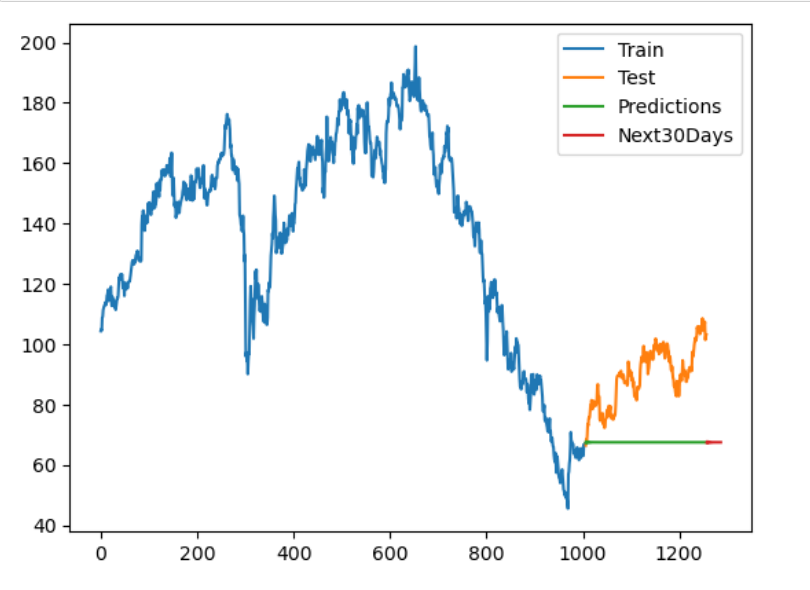
\includegraphics[max width=\linewidth, height = 4cm, center]{ARIMA_ADDYY_8-2.png}
Figure 4. Result of ARIMA with ADIDAS divided by 8-2 ratio.
\end{center}

\begin{table}[H]
\centering
\begin{tabularx}{\columnwidth}{|c|c|X|X|X|X|}
\hline
Model & \begin{tabular}{c}
Train- \\
Test
\end{tabular} & MSE & RMSE & MAE & MAPE \\
\hline
\multirow{3}{*}{ARIMA} & $7-3$ & 219.827 & 14.826 & 11.269 & 0.159 \\
\cline{2-6}
 & $8-2$ & 571.086 & 23.897 & 22.041 & 0.2378 \\
\cline{2-6}
 & $9-1$ & 40.729 & 6.381 & 22.041 & 0.0565 \\
\hline
\end{tabularx}
\end{table}

Table IV. ADIDAS measure result after using $ARIMA$.
\newline
\subsubsection*{\textbf{4) Seasonal Autoregressive Integrated Moving-Average with Exogenous Regressors (SARIMAX)}}
SARIMAX represents an extension of the ARIMA model, encompassing the incorporation of both seasonal patterns and external factors. Recognized for their robust forecasting capabilities, SARIMAX models are extensively applied in statistical forecasting and exhibit outstanding performance.

From the article by Fahad Radhi Alharbi and Denes Csala, the SARIMAX model consists of both seasonal effects and exogenous factors that can be used as SARIMAX (p, d, q) ∗ (P, D, Q), while the exogenous factors are optional parameters [15]
\[\phi_p(G)\phi_p(G^s)(1 - G)^d(1 - G^s)^D X_t = \alpha_k \gamma_{k,t} + \gamma_q(G)w_Q(G^s)e_t\]
\begin{itemize}
    \item \(\phi_p(G)\): Auto regressive function phi (AR) at lag p, where G is the time operator (lag operator)
    \item \(\phi_p(G^s)\): Seasonal auto regressive function (AR) at lag p, where \(G^s\) is the seasonal lag operator
    \item \((1 - G)^d\): The difference operator is at lag d, where d is the spatial difference.
    \item \((1 - G^s)^D\): The seasonal difference operator is at lag D, where D is the spatial seasonal difference.
    \item \(X_t\): Original data series or data series that are spatially and seasonally different.
    \item \(\alpha_k\): Coefficient of the autoregressive component phi (AR) at lag k
    \item \(\gamma_{k,t}\): Coefficient of the seasonal autoregressive component at lag k and time t.
    \item \(\gamma_q(G)\): Theta auto regressive function (MA) at lag q, where G is the time operator.
    \item \(w_Q(G^s)\): Seasonal theta auto regressive function at lag Q, where \(G^s\) is the seasonal time operator.
    \item \(e_t\): Random noise.

\end{itemize}
\begin{center}
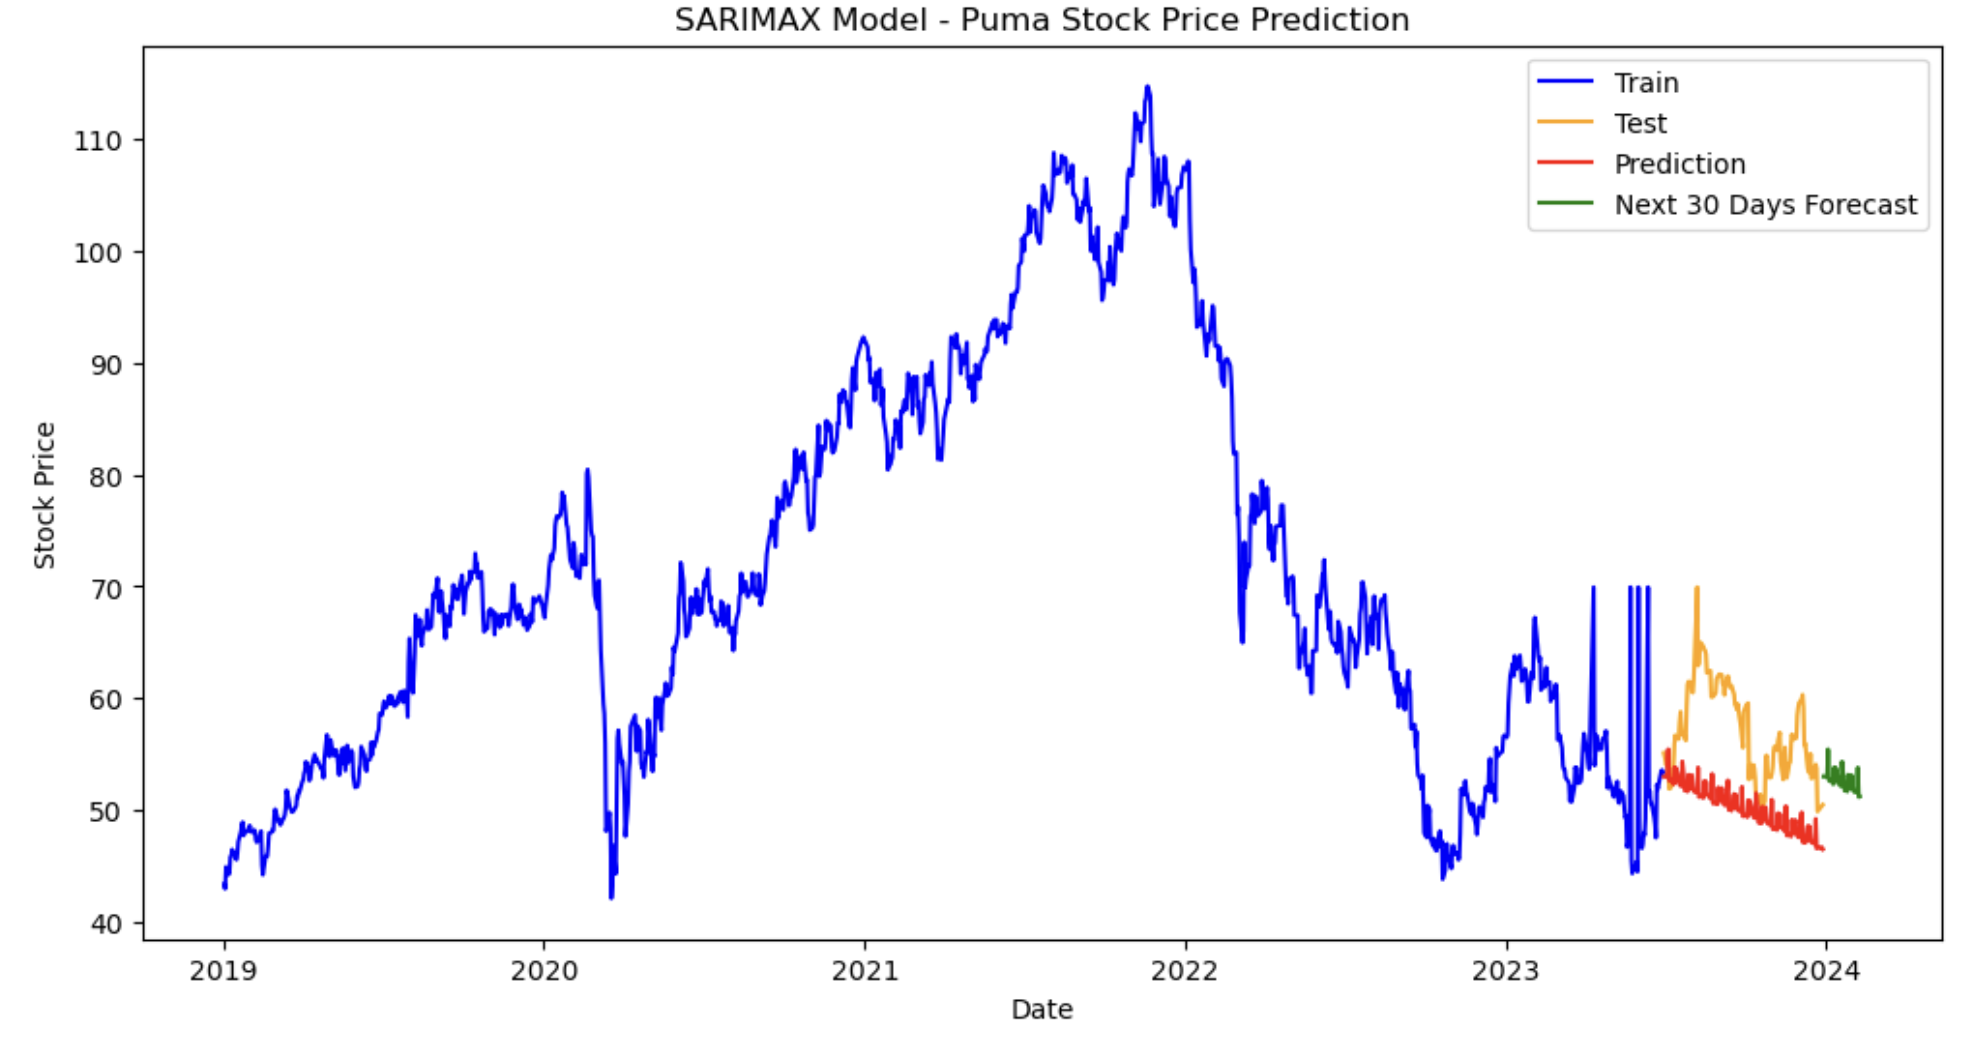
\includegraphics[max width=\linewidth]{SARIMAX(PUMA).png}
Figure 5. Result of SARIMAX with Puma divided by 9-1 ratio
\end{center}
\begin{table}[H]
\centering
\begin{tabularx}{\columnwidth}{|c|c|X|X|X|X|}
\hline
Model & \begin{tabular}{c}
Train- \\
Test
\end{tabular} & MSE & RMSE & MAPE & MAE \\
\hline
\multirow{3}{*}{SARIMAX} & $7-3$ & 125.55 & 11.21 & 18.60 & 9.84 \\
\cline{2-6}
 & $8-2$ & 26.59 & 5.16 & 7.48 & 4.21 \\
\cline{2-6}
 & $9-1$ & 63.70 & 7.98 & 12.10 & 7.12 \\
\hline
\end{tabularx}
\end{table}
Table V. Puma measure result after using $SARIMAX$.
\newline
\subsubsection*{\textbf{5) Kalman-Filter (KF)}}
Simply put, the Kalman Filter is a generic algorithm that is used to estimate system parameters. It can use inaccurate or noisy measurements to estimate the state of that variable or another unobservable variable with greater accuracy. For example, Kalman Filtering is used to do the following:

\begin{itemize}
  \item Object Tracking – Use the measured position of an object to more accurately estimate the position and velocity of that object. \\
  \item Body Weight Estimate on Digital Scale – Use the measured pressure on a surface to estimate the weight of object on that surface. \\
  \item Guidance, Navigation, and Control – Use Inertial Measurement Unit (IMU) sensors to estimate an objects location, velocity, and acceleration; and use those estimates to control the objects next moves. 
\end{itemize}
The real power of the Kalman Filter is not smoothing measurements. It is the ability to estimate system parameters that can not be measured or observed with accuracy. Estimates with improved accuracy in systems that operate in real time, allow systems greater control and thus more capabilities[16]. Here are the overview of the algorithm:
\begin{itemize}
  \item Initialize state estimate \(x_0\) and state covariance matrix \(P_0\) \\
  \item Predict System State and System State Error Covariance to Measurement Time 
\begin{align*}
\hat{x}_{k|k-1} &= F_k \hat{x}_{k-1|k-1} + B_k u_k \\
P_{k|k-1} &= F_k P_{k-1|k-1} F_k^T + Q_k
\end{align*} 
  \item Compute the Kalman Gain
  \begin{align*}
K_k &= P_{k|k-1} H_k^T (H_k P_{k|k-1} H_k^T + R_k)^{-1} \\
\end{align*}
\item Estimate System State and System State Error Covariance at Measurement Time
\begin{align*}
\hat{x}_{k|k} &= \hat{x}_{k|k-1} + K_k(z_k - H_k \hat{x}_{k|k-1}) \\
P_{k|k} &= (I - K_k H_k) P_{k|k-1}
\end{align*}
\end{itemize}
  \begin{flushleft}
    \textit{\textbf{Where:}}
    \begin{itemize}
      \item $\hat{x}_{k|k-1}$ is the predicted state estimate at time $k$
      \item $P_{k|k-1}$ is the predicted error covariance matrix at time $k$
      \item $K_k$ is the Kalman Gain
      \item $H_k^T$ is the transpose of the measurement matrix $H_k$
      \item $I$ represents the identity matrix
      \item $B_k$ is the control input vector
      \item $F_k$ is the state transition matrix.
      \item $Q_k$ represents the covariance matrix of the process noise at time $k$
      \item $u_k$ is the control input vector
      \item $z_k$ is the measurement vector at time $k$
    \end{itemize}
  \end{flushleft}
\begin{center}
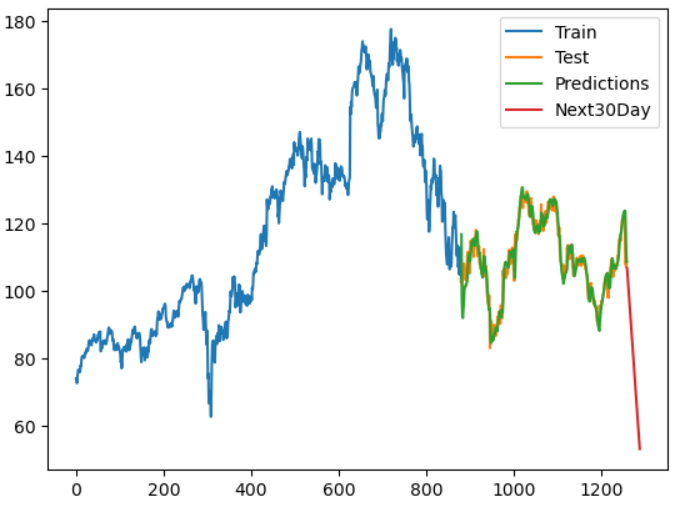
\includegraphics[ width=\linewidth]{Kalman.png}
Figure 6. Result of Kalman-Filter Model with NIKE divided by 7-3 ratio
\end{center}
\setlength{\parskip}{0pt}
\begin{table}[H]
\centering
\begin{tabularx}{\columnwidth}{|c|c|X|X|X|X|}
\hline
Model & \begin{tabular}{c}
Train- \\
Test
\end{tabular} & MSE & RMSE & MAPE & MAE \\
\hline
\multirow{3}{*}{Kalman-Filter} & $7-3$ & 9.7236 & 3.1182 & 2.0749 & 2.2334 \\
\cline{2-6}
 & $8-2$ & 5.9503 & 2.4393 & 1.6131 & 1.7967 \\
\cline{2-6}
 & $9-1$ & 8.0626 & 2.8394 & 1.8354 & 1.927 \\
\hline
\end{tabularx}
\end{table}
\setlength{\parskip}{0pt}
Table VI. NIKE measure result after using KF. \\
\setlength{\parskip}{0pt}
\subsubsection*{\textbf{6) Support Vector Regression (SVR)}}
SVR model is used to construct a composite scale in a specific zero dimension. This procedure involves input rays with no particular dimension and performs linear feature recovery in that space. The goal of SVR is to find a super-engineered linear feature that matches the input and output values. This model is then used to predict the output value during file inspection. The super method is defined by \textit{f}(\textit{x})=\textit{wx}+\textit{b}, 

Where w is the gradient and b is the error. SVR uses an epsilon-insensitive loss function to determine an acceptable range for the error. Parameter adjustment C decides the balance between model complexity and training accuracy. The goal of minimizing total risk includes training errors and complex models. Finally, to solve the problem of linear model performance when the relationship between input and output is nonlinear, SVR uses a function diagram ϕ to convert point data to a more specific zero height. [17]

\begin{table}[H]
    \centering
    \begin{tabular}{|c|c|} \hline 
         Kernel name& Formula\\ \hline 
         Linear& x^T_i x\\ \hline 
         Polynomial& (\gamma x^T_i x + r) ^ d\\ \hline 
         Radial Basis& e^-\gamma(||x_i - x||^2)\\ \hline 
         Sigmoidal& tanh(\gamma x^T_i x + r)\\ \hline
    \end{tabular}
    \label{tab:my_label}
\end{table}
Table VII: Overview of common kernel functions
\begin{itemize}
    \item \(\gamma\): is the scaling factor.
    \item r: is a constant coefficient.
    \item d: is the degree of the polynomial
\end{itemize}
SVR is a powerful regression technique, suitable for handling both linear and nonlinear relationships in data, providing flexibility through different kernel functions. The regularization parameter allows adjusting the balance between error and model complexity.
\begin{center}
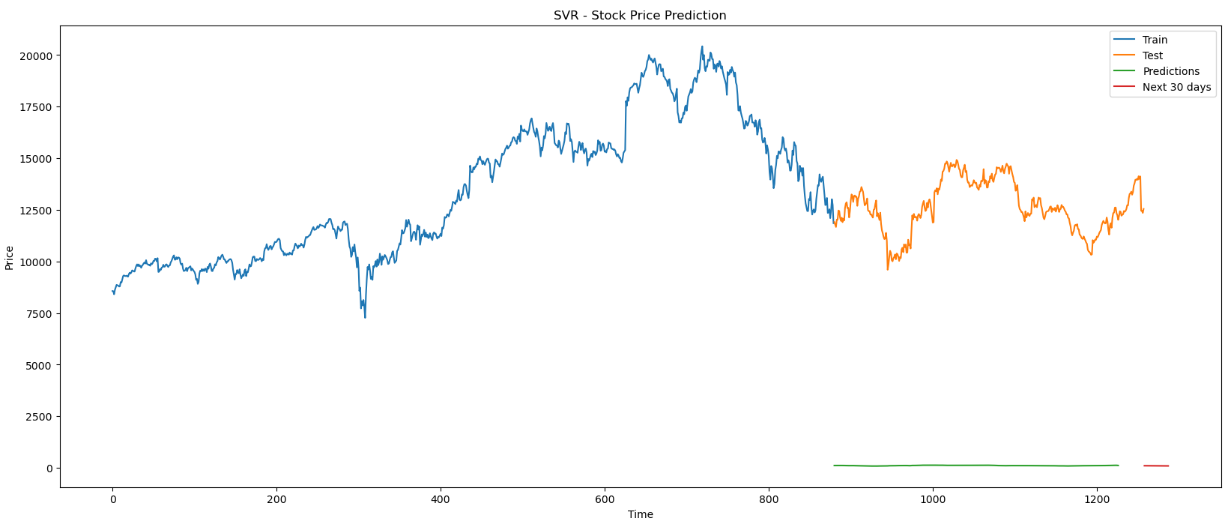
\includegraphics[max width=\linewidth]{SVR.png}
Figure 7. Result of SVR with Nike divided by 7-3 ratio
\end{center}
\begin{table}[H]
\centering
\begin{tabularx}{\columnwidth}{|c|c|X|X|X|X|}
\hline
Model & \begin{tabular}{c}
Train- \\
Test
\end{tabular} & MSE & RMSE & MAPE & MAE \\
\hline
\multirow{3}{*}{SVR} & $7-3$ & 0.00078 & 35.5703 & 0.05726 & 0.02169 \\
\cline{2-6}
 & $8-2$ & 0.00056 & 0.0238 & 0.04595 & 0.01835 \\
\cline{2-6}
 & $9-1$ & 0.00053 & 0.023 & 0.04835 & 0.01726 \\
\hline
\end{tabularx}
\end{table}
\setlength{\parskip}{0pt}
Table VIII. NIKE measure result after using SVR.\\
\subsubsection*{\textbf{7) Long-Short Term Memory (LSTM)}}
LSTM stands for long short-term memory networks, used in the field of Deep Learning. LSTM is a type of recurrent neural network that is capable of processing sequential data, making it a useful tool for analyzing time series data in the field of marketing.

LSTMs are explicitly crafted to overcome the challenge of long-term dependency. They inherently excel at retaining information over extended periods, a characteristic that comes naturally to them rather than being a challenging aspect to acquire!

All recurrent neural networks follow a pattern of consisting of repeated neural network modules. In conventional RNNs, these recurring modules are typically simplistic in structure, often comprising just a single tanh layer.

The essential components of LSTM include the memory cell and various gates (including the forget gate, input gate, and output gate). These gates determine which information needs to be added, erased, and output from the memory cell.[18]

\begin{center}
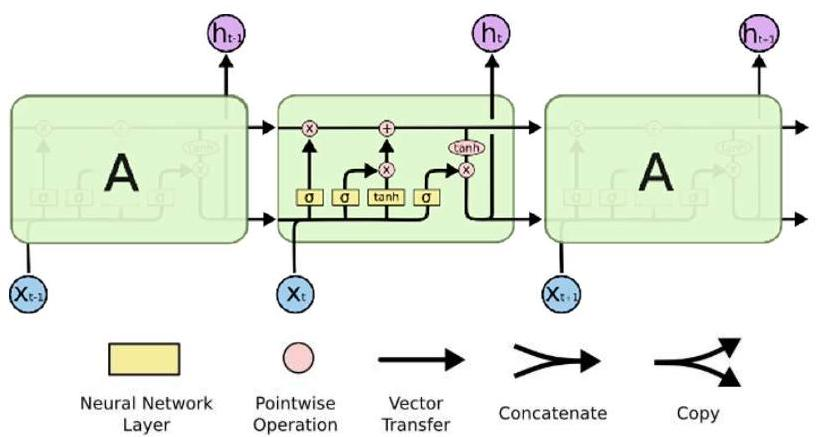
\includegraphics[max width=\linewidth, height = 5cm]{LSTM-architecture.jpg}
Figure 7. LSTM's Architecture
\end{center}

% Forget gate
The forget gate will discard information that is no longer useful from the memory cell. The equation for the forget gate is:
\[ f_t = \sigma(W_f [h_{t-1}, x_t] + b_f) \]

\textbf{Where:}
\begin{itemize}
    \item $\sigma$ is the sigmoid activation function.
    \item $W_f$ and $b_f$ are the weights and biases of the forget gate.
\end{itemize} 
% Input gate
The input gate will add useful information to the memory cell. The equation for the input gate is:
\[ i_t = \sigma(W_i [h_{t-1}, x_t] + b_i) \]
\[ \tilde{C}_t = \tanh(W_C [h_{t-1}, x_t] + b_C) \]
\[ C_t = f_t \ast C_{t-1} + i_t \ast \tilde{C}_t \]

\textbf{Where:}
\begin{itemize}
    \item $\sigma$ is the sigmoid activation function.
    \item $W_i$ and $b_i$ are the weights and biases of the input gate.
    \item $\tilde{C}_t$ is the modified input.
\end{itemize}

% Output gate
The output gate will extract useful information from the current memory cell to be presented as output. The equation for the output gate is:
\[ o_t = \sigma(W_o [h_{t-1}, x_t] + b_o) \]

\textbf{Where:}
\begin{itemize}
    \item $\sigma$ is the sigmoid activation function.
    \item $W_o$ and $b_o$ are the weights and biases of the output gate.
\end{itemize}

\begin{center}
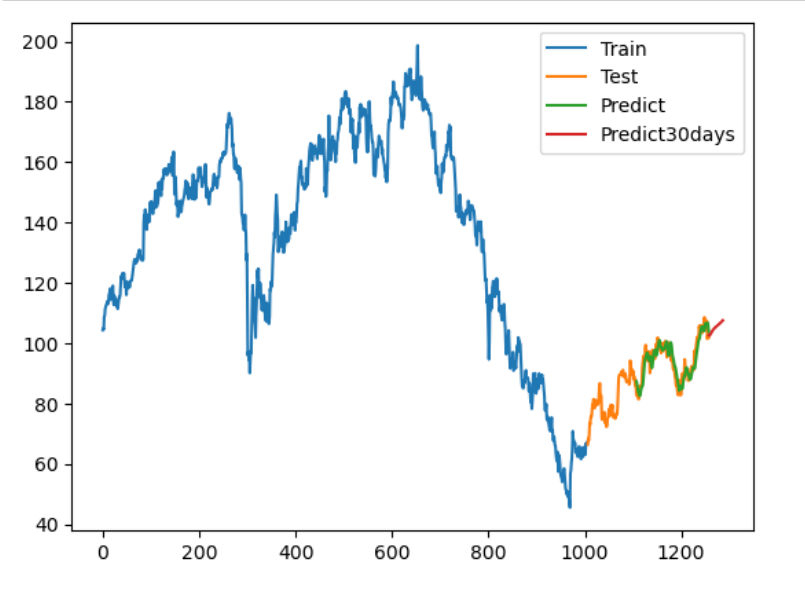
\includegraphics[max width=\linewidth]{LSTM_ADDYY_8-2.png}
\end{center}

Figure 8. Result of LSTM with ADIDAS divided by 8-2 ratio.

\begin{table}[H]
\centering
\begin{tabularx}{\columnwidth}{|c|c|X|X|X|X|}
\hline
Model & \begin{tabular}{c}
Train- \\
Test
\end{tabular} & MSE & RMSE & MAE & MAPE \\
\hline
\multirow{3}{*}{LSTM} & $7-3$ & 7707.597 & 87.802 & 87.03227 & 339.3455 \\
\cline{2-6}
 & $8-2$ & 8694.9853 & 93.249 & 93.032 & 292.166 \\
\cline{2-6}
 & $9-1$ & 10380.352 & 101.884 & 101.860 & 265.163 \\
\hline
\end{tabularx}
\end{table}

Table IX. ADIDAS measure result after using $LSTM$.
\newline
\subsubsection*{\textbf{8) Bagging Gated Recurrent Unit (Bagging-GRU)}}
Bagging is the type of ensemble technique in which a single training algorithm is used on different subsets of the training data where the subset sampling is done with replacement (bootstrap). Once the algorithm is trained on all the subsets, then bagging makes the prediction by aggregating all the predictions made by the algorithm on different subsets. In the context of GRU (Gated Recurrent Unit), bagging involves training multiple GRU models on different subsets of the training data and then combining their predictions.

When bagging is applied to GRU models, each individual GRU model is trained independently on a subset of the data, and their predictions are aggregated to produce a more robust and accurate prediction. This technique is commonly used in machine learning, including with recurrent neural networks like GRU and LSTM (Long Short-Term Memory).[19]

\begin{center}
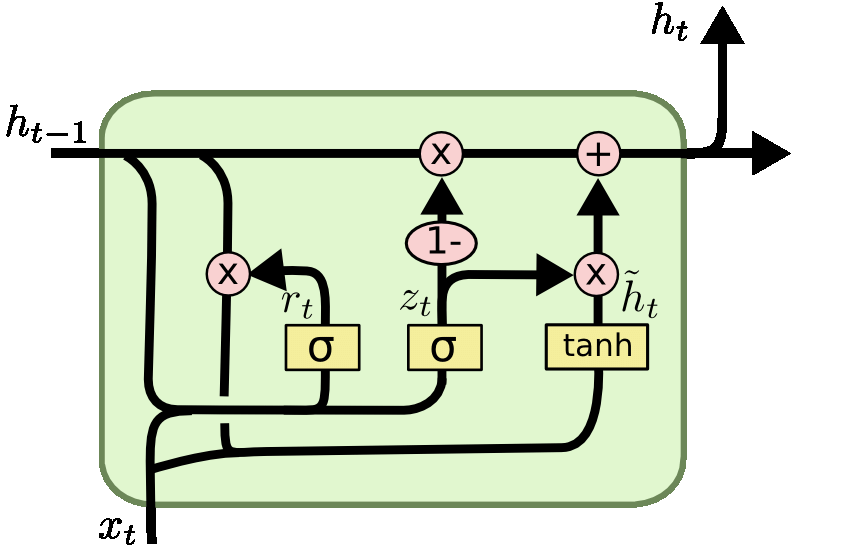
\includegraphics[max width=\linewidth, height = 4cm]{Gated-Recurrent-Unit-GRU.png}
\end{center}

Figure 9. GRU's Architecture\\
\begin{table*} 
    \centering
    \resizebox{\textwidth}{!}{%
        \begin{tabular}{|l|l|S[table-format=4.4]|S[table-format=2.4]|S[table-format=1.5]|S[table-format=2.4]|S[table-format=4.4]|S[table-format=2.4]|S[table-format=1.4]|S[table-format=2.4]|S[table-format=4.4]|S[table-format=2.4]|S[table-format=1.4]|S[table-format=2.4]|}
            \hline
            \multirow{2}{*}{Brands} & \multicolumn{1}{c|}{\multirow{2}{*}{Models}} & \multicolumn{4}{c|}{Test set (7-3)} & \multicolumn{4}{c|}{Test set (8-2)} & \multicolumn{4}{c|}{Test set (9-1)} \\ \cline{3-14}
            & & {MSE} & {RMSE} & {MAPE} & {MAE} & {MSE} & {RMSE} & {MAPE} & {MAE} & {MSE} & {RMSE} & {MAPE} & {MAE} \\ \hline
            \multirow{8}{*}{NIKE}   & Linear Regression                            & 4525.8352 & 67.2743 & 0.61408 & 65.6534 & 1503.5107 & 38.7751 & 0.3372 & 36.4513 & 1331.7886 & 36.4936 & 0.3468 & 35.7974 \\ \cline{2-14} 
                        & SES                                          & 126.06 & 11.23 & 8.73 & 9.43 & 268.93 & 16.40 & 12.75 & 13.41 & 167.35 & 12.94    & 11.18 & 11.28     \\ \cline{2-14} 
                        & ARIMA                                      & 160.81804 & 12.6814 & 0.091 & 10.3729 & 129.7126  & 11.389 & 0.0898 & 9.5635 & 121.904 & 11.04101 & 0.094 & 9.50608  \\ \cline{2-14} 
                        & SARIMAX                                      & 126.38 & 11.24 & 8.78 & 9.45 & 266.54 & 16.33 & 12.70 & 13.37 & 164.10 & 12.81 & 11.06 & 11.15     \\ \cline{2-14} 
                        & Kalman-Filter                                & 9.7236 & 3.118 & 2.074 & 2.2334 & 5.9503 & 2.4393 & 1.6131 & 1.7967 & 8.0626 & 2.8394 & 1.8354 & 1.927 \\ \cline{2-14} 
                        & SVR                                          & 0.00078 & 0.02793 & 0.05726 & 0.02169 & 0.00056 & 0.0238 & 0.04595 & 0.01835 & 0.00052 & 0.023 & 0.048 & 0.0172  \\ \cline{2-14} 
                        & LSTM                                         &  12227.304 & 110.5842 &  262.2129 & 110.1747 & 11336.87 & 106.478 & 288.64 & 106.252 & 13021.384 &  114.113 & 254.7002 & 113.972 \\ \cline{2-14} 
                        & Bagging-GRU                                  & \textbf{0.00033} & \textbf{0.0181} & \textbf{0.0302} & \textbf{0.0125} & \textbf{0.00029}  & \textbf{0.0172} & \textbf{0.0273} & \textbf{0.01204} & \textbf{0.00026} & \textbf{0.0161} &\textbf{ 0.025} & \textbf{0.0109}   \\ \hline
            \multirow{8}{*}{ADIDAS} & Linear Regression                            & 695.1086 & 26.3701 & 0.3528 & 25.0136 & 448.5993 & 21.1772 & 0.2577 & 19.7483  & 233.7345 & 15.3011  & 0.2087  & 13.8907 \\ \cline{2-14} 
                        & SES                                          & 168.93 & 13.00 & 11.62 & 12.17 & 362.84 & 19.05 & 18.85  & 18.95 & 221.88 & 14.90 & 13.42 & 14.00     \\ \cline{2-14} 
                        & ARIMA                                        & 299.72542 & 17.316 & 0.12543 & 14.5159 & 222.9387 & 14.9442 & 0.1234 & 13.0915 & 194.85853 & 13.96864 & 0.12868 & 12.8701  \\ \cline{2-14} 
                        & SARIMAX                                      & 166.96 & 12.92 & 11.56 & 12.04 & 353.42 & 18.78 & 18.53 & 18.62 & 209.24 & 14.47 & 13.21 & 14.05     \\ \cline{2-14} 
                        & Kalman-Filter                                & 41.0948  & 6.4105  & 3.605 & 2.939 & 83.382 & 9.1313 & 4.5485 & 3.6227  & 42.8387 & 6.5451 & 3.5162 & 3.3498  \\ \cline{2-14} 
                        & SVR                                          & 0.00058 & 0.02415 & 0.0473 & 0.0192 & 0.00044 & 0.021 & 0.0386 & 0.016  & 0.00039 & 0.01985 & 0.03678 & 0.01577   \\ \cline{2-14} 
                        & LSTM                                         & 7144.9102 & 84.5193 & 203.06 & 83.95 & 6767.696 & 82.241 & 223.72 & 81.9897 & 8665.29 & 93.102 & 182.697 & 92.769  \\ \cline{2-14} 
                        & Bagging-GRU                                  & \textbf{0.00023 }&\textbf{ 0.0152 }& \textbf{0.0261} & \textbf{0.0109} & \textbf{0.00019} & \textbf{0.0137} & \textbf{0.0217} & \textbf{0.0094} & \textbf{0.00017} & \textbf{0.0131} & \textbf{0.02077} & \textbf{0.0087}  \\ \hline
            \multirow{8}{*}{PUMA}   & Linear Regression                            & 2696.981 & 51.9324  & 0.9326 & 51.1719 & 939.3682 & 30.6491 & 0.54849 & 30.1936  & 315.0609  & 17.749 & 0.3086 & 17.2998  \\ \cline{2-14} 
                        & SES                                          & 128.94 & 11.36 & 18.87 & 9.98 & 32.18 & 5.67 & 8.76 & 4.79 & 28.47 & 5.34 & 7.03 & 4.20      \\ \cline{2-14} 
                        & ARIMA                                        & 99.8815 & 9.994 & 0.16177 & 8.4366  & 24.8734 & 4.9873  & \textbf{0.07171} & 4.06964 & 29.6833 & 5.4482 & \textbf{0.07276} & 4.34539  \\ \cline{2-14} 
                        & SARIMAX                                      & 125.55 & 11.21   & 18.60 & 9.84 & 26.59 & 5.16 & 7.48 & 4.21 & 63.70 & 7.98 & 12.10 & 7.12      \\ \cline{2-14} 
                        & Kalman-Filter                                & 4.9298   & 2.2203 & 2.7169 & 1.5435 & 8.5046 & 2.9162& 3.1133& 1.7457 & 11.9116 & 3.4513 & 3.6959 & 2.0578 \\ \cline{2-14} 
                        & SVR &0.0007 & 0.02672 & 0.15409 & 0.0217 & 0.00069 & 0.02637 & 0.14204& 0.0213 & 0.0005  & 0.02354 & 0.1005 & 0.01795   \\ \cline{2-14} 
                        & LSTM                                         & 3187.2187  & 56.460 & 348.1532 & 56.291 &  3156.56 & 56.188 & 360.6178 & 55.985 & 3161.0455 & 56.224 &   317.281 & 56.175  \\ \cline{2-14} 
                        & Bagging-GRU                      & \textbf{0.00038} & \textbf{0.0196} & \textbf{0.100992} & \textbf{0.0147} &\textbf{0.00039} & \textbf{0.01995} & 0.1068 & \textbf{0.0145} & \textbf{0.00039} & \textbf{0.01999} & 0.087 & \textbf{0.0142}  \\ \hline
        \end{tabular}%
    }
    \label{tab:my-table}
\end{table*}
\begin{center}
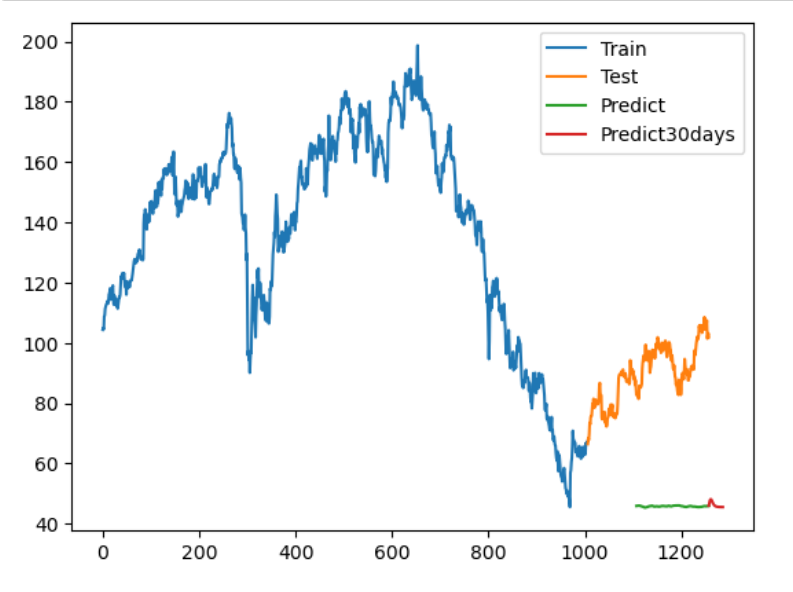
\includegraphics[max width=\linewidth]{B-GRU_ADDYY_8-2.png}
Figure 10. Result of Bagging-GRU with ADIDAS divided by 8-2 ratio.
\end{center}
\begin{table}[H]
\centering
\begin{tabularx}{\columnwidth}{|c|c|X|X|X|X|}
\hline
Model & \begin{tabular}{c}
Train- \\
Test
\end{tabular} & MSE & RMSE & MAE & MAPE \\
\hline
\multirow{3}{*}{B-GRU} & $7-3$ & 0.000163 & 0.012 & 0.0093 & 0.0299 \\
\cline{2-6}
 & $8-2$ & 0.000157 & 0.0125 & 0.0094 & 0.0299 \\
\cline{2-6}
 & $9-1$ & 0.00015 & 0.01228 & 0.0088 & 0.023 \\
\hline
\end{tabularx}
\end{table}
Table X. ADIDAS measure result after using $Bagging-GRU$


\section*{IV. Experimental results} 
The performance evaluation results of time series forecasting methods on the test set are shown in Table II. Overall, deep learning network models show outstanding performance compared to traditional time series forecasting models based on Machine Learning. Besides Linear Regression, the standard ARIMA model shows the lowest experimental performance among the methods on all 5 measures because it does not use seasonal characteristics, so the forecast line is only straight line. Based on the RMSE measure, the predictions of the models when using the ratio 7:3 for the experimental process often show better evaluation performance than when using 8:2 and 9:1 on all three. Nike, Puma, and Adidas stores.

\section*{V. Conclusion}

In our research on stock price forecasting, we applied 8 different algorithms, including Linear Regression, SARIMAX, KF, SES, ARIMA, LSTM, SVR, Bagging GRU, to forecast stock prices for 30 days coming from three fashion stores: Nike, Puma, Adidas. The results show that statistical models often outperform traditional machine learning models in time series forecasting.

For the Adidas store at 8:2 ratio, the LSTM model achieved the best performance. For the 9:1 ratio Puma store, the SARIMAX model achieved the highest performance. For the Nike store at 7:3 ratio, the Kalman filter model achieved the best performance.

Despite its positive contributions, the study also has limitations such as not conducting certain preprocessing steps and lacking optimization of the model and method. In the future, we will continue to research and overcome these limitations, as well as consider additional environmental factors such as temperature and salinity to improve forecasts.

\section*{VI.ACKNOWLEDGMENT}
\selectlanguage{vietnamese}

First and foremost, we extend our sincere thanks to Assoc.Prof. Dr. Nguyễn Đình Thuân. We are grateful for his insightful lectures and enthusiastic guidance, which have equipped the team with the knowledge needed to successfully complete the project. Our heartfelt thanks also go to Mr. Nguyễn Minh Nhựt for his unwavering support throughout the course.

We would like to express our gratitude to Assoc.Prof. Dr. Nguyễn Đình Thuân for granting us permission to undertake our project.

Finally, we want to convey our deep appreciation to Assoc.Prof. Dr. Nguyễn Đình Thuân and Mr. Nguyễn Minh Nhựt for their tireless efforts in mentoring the team throughout the project and for motivating us to persist in our endeavors.

\section*{VII.REFERENCES}
[1] 1. Moon TS, Van de Putte P, De Baerdemaeker L, Schumann R. The obese patient: facts, fables and best practices. Anesth Analg. 2021;132:53–64.

[2],[15] Fahad Radhi Alharbi  and Denes Csala, "A Seasonal Autoregressive Integrated Moving Average with Exogenous Factors (SARIMAX) Forecasting Model-Based Time Series Approach", School of Engineering, Lancaster University, Lancaster LA1 4YR, UK

[3],[17] Mathieu Wauters , Mario Vanhoucke, "Support Vector Machine Regression for project control forecasting", Faculty of Economics and Business Administration, Ghent University, Tweekerkenstraat 2, 9000 Gent (Belgium)

[4] Everette S. Gardner Jr, "Exponential smoothing: The state of the art—Part II", Bauer College of Business, 334 Melcher Hall, University of Houston, Houston, TX 77204-6021, United States

[5] Hyndman, R. J.,  Athanasopoulos, G. (2018). Forecasting: Principles and Practice. OTexts, Vol. 1, pp. 56-78.

[3] Hastie, T., Tibshirani, R.,  Friedman, J. (2009). The Elements of Statistical Learning: Data Mining, Inference, and Prediction. Springer, Vol. 3, pp. 200-225.

[6] "NIKE, Inc. (NKE) \href{https://finance.yahoo.com/lookup?s=DATA}{finance.yahoo.com}." \href{https://finance.yahoo.com/quote/NKE/history?period1=1546128000&period2=1703894400&interval=1d&filter=history&frequency=1d&includeAdjustedClose=true}{NIKE}. (accessed Dec. 30, 2023).

[7] "PUMA SE (PUM.DE) \href{https://finance.yahoo.com/lookup?s=DATA}{finance.yahoo.com}." \href{https://finance.yahoo.com/quote/PUM.DE/history?period1=1546128000&period2=1703894400&interval=1d&filter=history&frequency=1d&includeAdjustedClose=true}{PUMA} (accessed Dec. 30, 2023).

[8] "adidas AG (ADDYY) \href{https://finance.yahoo.com/lookup?s=DATA}{finance.yahoo.com}." \href{https://finance.yahoo.com/quote/ADDYY/history?period1=1546128000&period2=1703894400&interval=1d&filter=history&frequency=1d&includeAdjustedClose=true}{ADIDAS} (accessed Dec. 30, 2023).

[9] MSE, RMSE, MAE \href{https://medium.com/analytics-vidhya/mae-mse-rmse-coefficient-of-determination-adjusted-r-squared-which-metric-is-better-cd0326a5697e}{MAE, MSE, RMSE, Coefficient of Determination, Adjusted R Squared — Which Metric is Better?}.(accessed Dec. 21, 2023).

[10] MAPE \href{https://www.indeed.com/career-advice/career-development/what-is-mape}{What Is MAPE? A Guide to Mean Absolute Percentage Error}.(accessed Dec. 21, 2023)

[11] "About Linear Regression | IBM." \href{https://www.ibm.com/topics/linear-regression}{What is Linear Regression ?} (accessed Dec. 20, 2023).

[12] "Everything you need to Know about Linear Regression!" \href{https://www.analyticsvidhya.com/blog/2021/10/everything-you-need-to-know-about-linear-regression/}{Simple Linear Regression} (accessed Dec. 20, 2023).

[13] \href{https://www.amazon.com/Nicolas-Vandeput/e/B07KL86HMV/ref=dp_byline_cont_book_1}{Nicolas Vandeput}, " Data Science for Supply Chain Forecasting 2nd Edition", 

[14] "Autoregressive Integrated Moving Average (ARIMA)," Corporate Finance Institute. \href{https://corporatefinanceinstitute.com/resources/datascience/autoregressive-integrated-moving-average-arima/}{AutoRegressive Integrated Moving Average-ARIMA/} (accessed Dec. 22, 2023).

[16] "Kalman-Filter," \href{https://thekalmanfilter.com/kalman-filter-explained-simply/}{Kalman Filter Explained Simply} (accessed Dec. 21, 2023).

[18] "Understanding LSTM Networks," [Online]. Available: \href{http://colah.github.io/posts/2015-08-Understanding-LSTMs/}{Understanding LSTM Networks}(accessed Dec. 22, 2023)

[19] "Ensemble Techniques, Ensemble Learning in Machine Learning Explanation," [Online]. Available: \href{https://pradeep-dhote9.medium.com/ensemble-techniques-ensemble-learning-in-machine-learning-explanation-cbc6b6a0bbf3}{Ensemble Techniques, Ensemble Learning




\end{document}